\section{Research Design and Methodology}
This study employs a mixed-methods approach, integrating both quantitative and qualitative research techniques to investigate the trade-offs between productivity and security in AI-assisted software development. By combining developer surveys, literature review, and code security analysis, the study aims to quantify and contextualize the security risks associated with AI-generated code while assessing their impact on development efficiency.

\subsection{Hypotheses}

To systematically investigate the research questions, the study formulates hypotheses only for those questions that involve measurable perceptions or effectiveness, specifically RQ1 and RQ2.1.

\subsubsection{For RQ1 (Perception of Trade-Offs)}

\begin{itemize}
    \item \textbf{H$_{0}$ (Null Hypothesis)}: Developers do not perceive a significant trade-off between speed and security when using AI-assisted coding tools.
    \item \textbf{H$_{1}$ (Alternative Hypothesis)}: Developers perceive a significant trade-off between speed and security when using AI-assisted coding tools.
\end{itemize}

\subsubsection{For RQ2 (What are the existing security verification practices)}

RQ2 is exploratory in nature and aims to identify and categorize existing practices. Therefore, it is not associated with a testable hypothesis but will be addressed through a structured literature and tool review.

\subsubsection{For RQ2.1 (Effectiveness of security verification practices)}

\begin{itemize}
    \item \textbf{H$_{0}$ (Null Hypothesis)}: Existing security verification practices are not effective in identifying vulnerabilities in AI-generated code.
    \item \textbf{H$_{1}$ (Alternative Hypothesis)}: Existing security verification practices are effective in identifying vulnerabilities in AI-generated code.
\end{itemize}

\subsection{Research Method}

\subsubsection{Developer Survey}

The survey will target 40-50 software developers, including 20 web developers, 5 test engineers, 5 DevOps engineers, and 10 backend developers, who actively use AI coding tools. It is designed to capture developers' perspectives on trade-offs between development speed and security risks, as well as their mitigation strategies.

Survey participants will be asked to indicate their level of agreement with various statements using a 5-point Likert scale, supplemented with open-ended questions for qualitative insights.

\paragraph{Survey Statements:}
\begin{itemize}
    \item AI tools help me write code faster, but I worry they introduce security risks.
    \item The time saved by using AI tools outweighs the effort required to fix security issues in AI-generated code.
    \item I prioritize code security over development speed when using AI tools.
    \item AI tools make it harder to follow secure coding practices (e.g., input sanitization, secure authentication).
    \item I feel pressured to deliver code quickly when using AI tools, even if it means compromising security.
\end{itemize}

\paragraph{Follow-Up Questions:}
\begin{itemize}
    \item What percentage of time saved by AI tools is spent fixing security issues?
    \item When using AI tools, how often do you review generated code for security flaws?
    \item Describe a situation where you had to choose between development speed and code security while using AI tools.
\end{itemize}

These responses will help quantify perceptions of security risks, assess common mitigation practices, and evaluate whether AI-generated efficiency gains are offset by additional security verification work.


\begin{figure}[H]
    \centering
    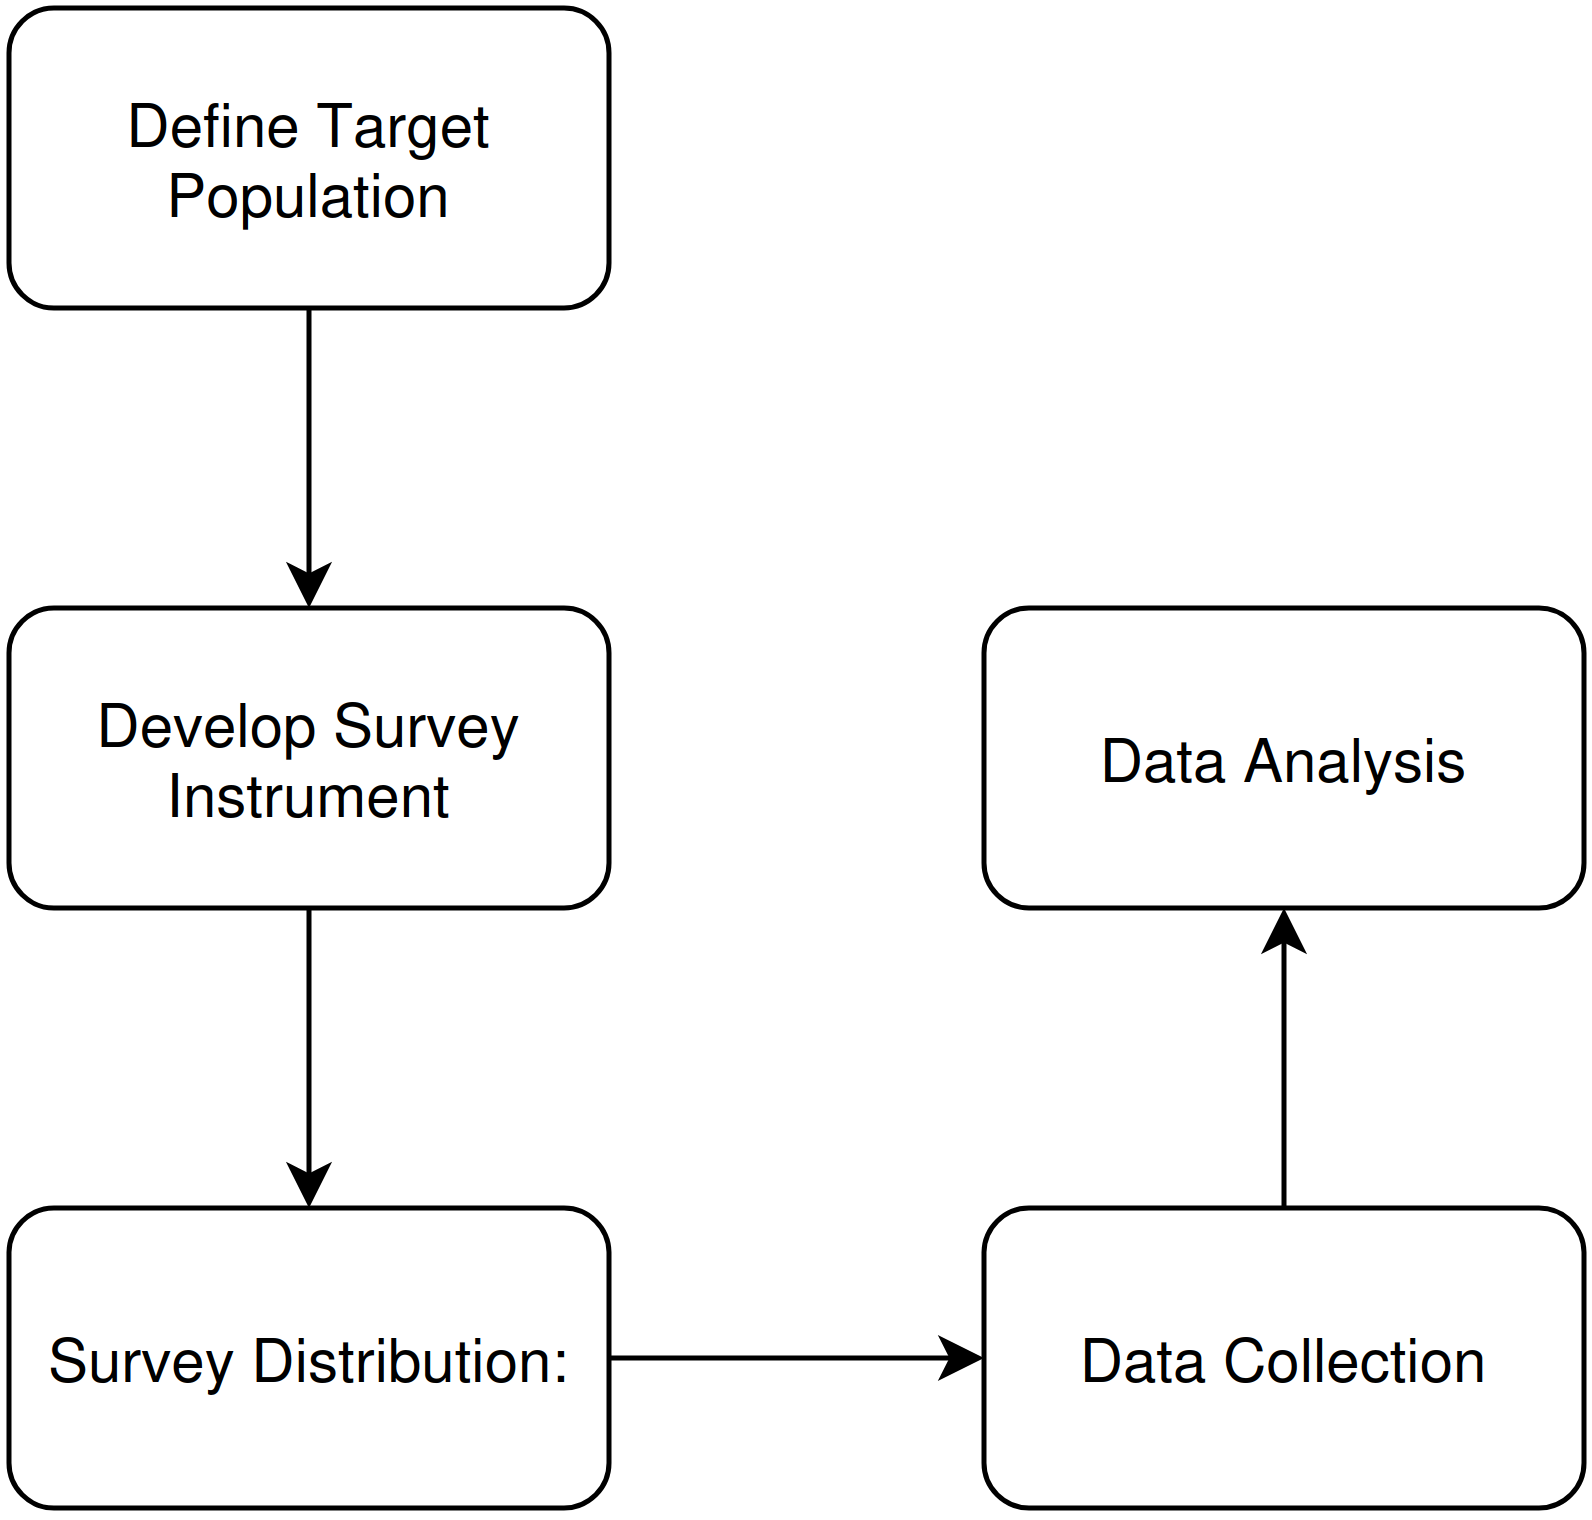
\includegraphics[width=0.9\columnwidth]{assets/survay-workflow.png}
    \caption{Workflow for the process of thesis's Developer Survey Research Method.}
    \label{fig:workflow_diagram}
\end{figure}


\subsubsection{Security Verification}
Landscape Review: To address the question of what security verification practices currently exist for AI-generated code, this section will review academic publications, industry reports, and documentation from security tools. The goal is to map out the landscape of available methods, examining their design, purpose, and level of automation. The review will pay particular attention to whether these methods were developed with AI-generated code in mind, and how they are integrated into modern development workflows. It will also highlight any gaps in existing practices such as overreliance on post-generation manual review that could hinder the secure adoption of AI coding tools. This investigation will provide the necessary context for evaluating the novelty and limitations of current security approaches in relation to the rapid pace of AI code generation.

\subsubsection{Code Analysis}

We will compile a dataset of 9-13 AI-generated code samples by utilizing various AI coding tools and sourcing existing publicly online available examples across multiple programming languages (e.g., Python, JavaScript, Java) and use cases (e.g., web development, API security, cryptographic functions). The selected samples will represent realistic coding scenarios to facilitate an in-depth security analysis.
The methodology for security analysis includes:

\begin{itemize}
    \item \textbf{Static Analysis} – Using industry-standard tools (e.g., SonarQube, Bandit, ESLint Security Plugin) to detect potential vulnerabilities automatically.
    \item \textbf{Manual Code Review} – Conducting expert analysis of AI-generated code to identify security flaws missed by automated tools, using OWASP guidelines and secure coding principles.
    \item \textbf{Severity Classification} – Categorizing vulnerabilities based on severity (low, medium, high) and type (e.g., SQL injection, insecure authentication, hardcoded secrets).
\end{itemize}

By examining patterns in security flaws and comparing them with survey responses, this analysis provides a direct measure of security trade-offs and how developers perceive and mitigate AI-generated risks.


\begin{figure}[H]
    \centering
    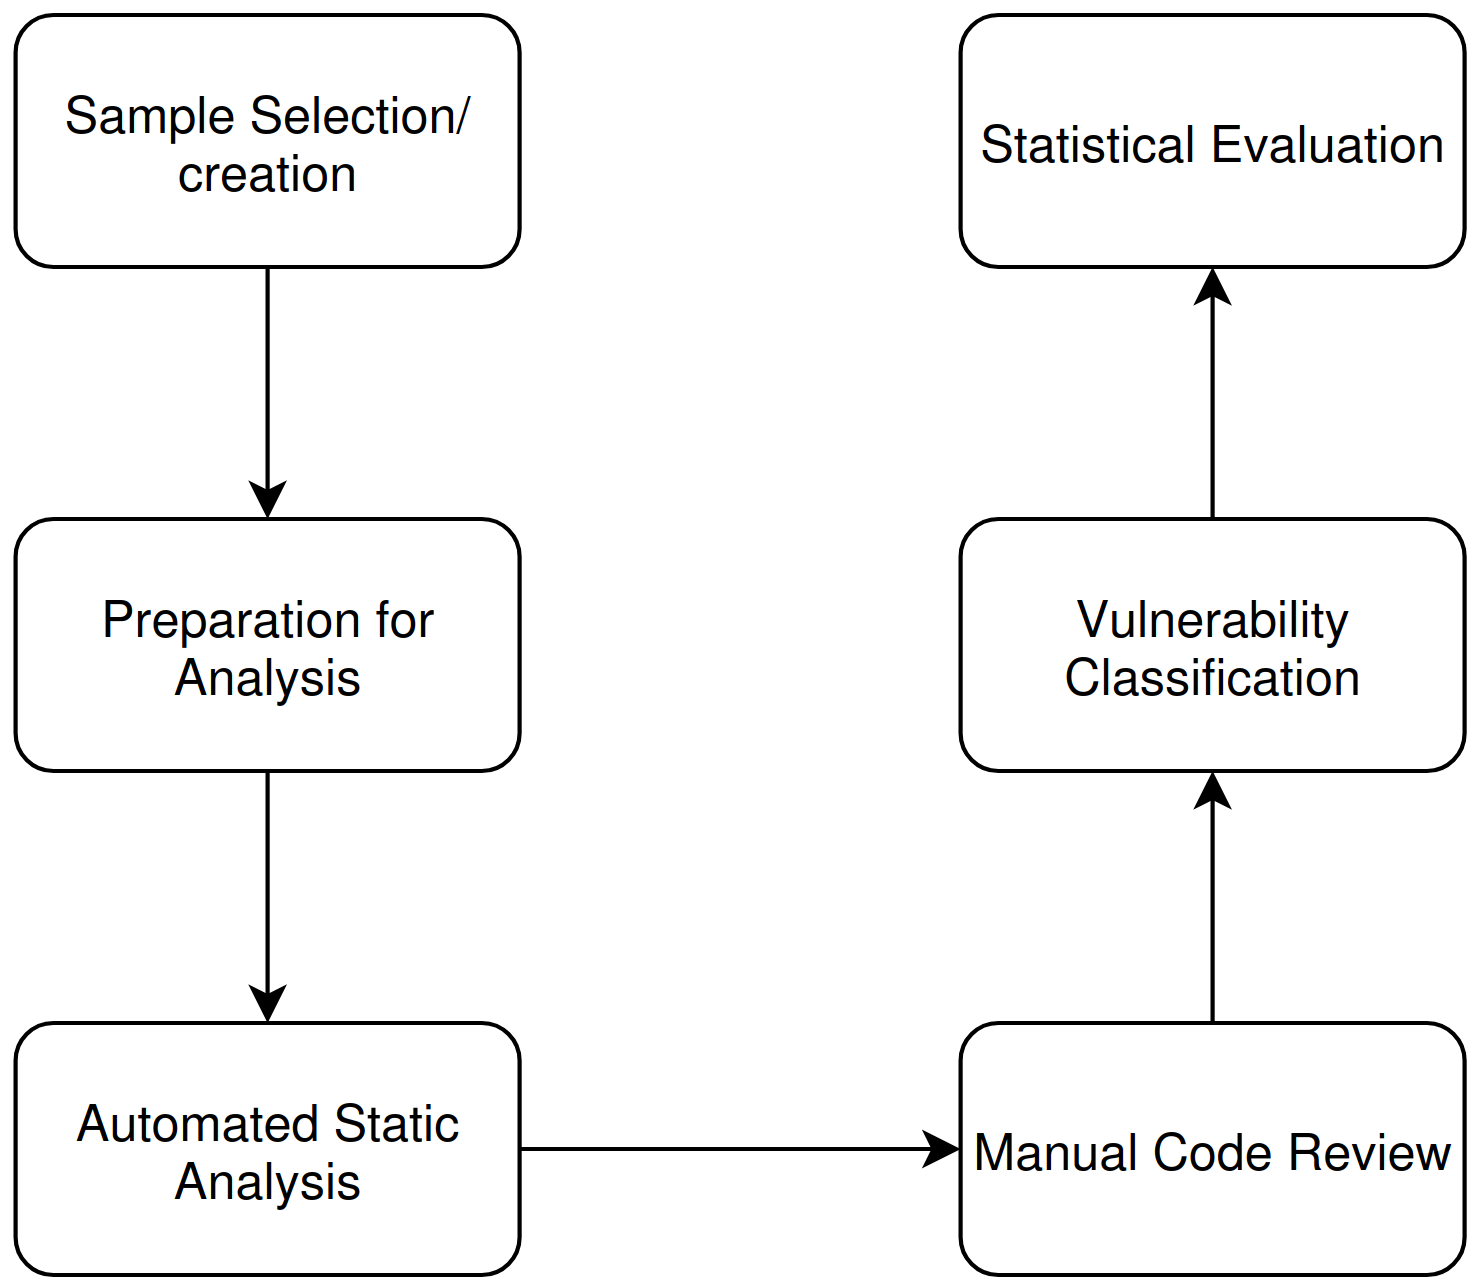
\includegraphics[width=0.9\columnwidth]{assets/data-analysis.png}
    \caption{Workflow for the process of thesis's Code Analysis Research Method.}
    \label{fig:data_analysis_diagram}
\end{figure}

\subsubsection{Code Sample Selection}
To ensure a balanced and representative dataset, code samples will be selected using a combination of randomized and purposeful sampling methods, adhering the following selection criteria:

\begin{itemize}
    \item \textbf{Programming Languages}: JavaScript, Java, c++, Python.
    \item \textbf{Types of Applications}: Web apps, APIs, cryptographic functions, data processing, authentication systems.
    \item \textbf{AI Tools Used}: GitHub Copilot, ChatGPT, AWS CodeWhisperer, Google Gemini.
    \item \textbf{Complexity}: Moderate complexity, code snippet, standalone components.
    \item \textbf{Randomized selection  (70\% of the samples, 5-7 samples)}: Randomly generated code snippets from common developer communities such as GitHub, Stack Overflow, AI code generation examples publicly shared by developers, and our own AI-generated examples using standard prompts, which if happened the prompts and conversation will be available to view.
    \item \textbf{Purposeful selection (30\% of your samples, 4-6 samples)}: Intentionally selecting a few samples:
    \begin{itemize}
        \item Known faulty examples: AI-generated code publicly flagged for vulnerabilities or security issues.
        \item Known clean examples: AI-generated code recognized or peer-reviewed as secure or adhering closely to security best practices.
        \item Popular scenarios from well-documented sources to represent standard industry practices (e.g., OWASP-related implementations).
    \end{itemize}
\end{itemize}

\begin{table}[h!]
    \caption{Sample Selection Criteria}
    \centering
    \renewcommand{\arraystretch}{1.4}
    \begin{tabular}{|l|l|}
    \hline
    \textbf{{Criteria}} & \textbf{{Number of samples}} \\
    \hline
    Randomly selected & 5-7 \\
    \hline
    Intentionally faulty & 2-3 \\
    \hline
    Intentionally clean & 2-3 \\
    \hline
    Total samples & 9-13 \\
    \hline
    Programming Languages & At least 3 (Python, JS, Java) \\
    \hline
    AI Generation Tools & At least 2 (Copilot, ChatGPT) \\
    \hline
    \end{tabular}
\end{table}
\vspace{-0.8em} 
\small\textit{A more detailed structure specifying the functionality, corresponding test cases, the version of the AI generation tool used, and the total number of samples for each programming language and AI tool will be provided at a later stage.}

\textbf{Justification of sample selection}
The dataset should represent realistic scenarios that reflect common developer practices and include but are not limited to languages commonly used, not just extremes of faulty or perfect code. Randomized Selection: Prevents bias, reflecting general AI usage realistically. Purposeful Selection: Captures extremes for detailed comparison and identifying recurring patterns or exceptions in vulnerabilities.

\subsection{Data Analysis}

\subsubsection{Survey Data}

Survey responses will be analyzed using statistical methods, including:

\begin{itemize}
    \item \textbf{Descriptive Statistics}: Mean, median, and standard deviation will be calculated for Likert-scale responses to summarize general trends in perceptions of AI-generated code security and efficiency.
    \item \textbf{Correlation Analysis}: Pearson or Spearman correlation tests will be used to identify relationships between developers’ concerns about security risks and their reported efficiency gains.
    \item \textbf{Comparative Analysis}: Independent t-tests or ANOVA will be applied to compare responses across different groups (e.g., experience levels, programming languages used) to assess variation in perceptions.
    \item \textbf{Thematic Analysis}: Open-ended responses will be categorized using thematic coding to extract qualitative insights on developers' security concerns and mitigation strategies.
\end{itemize}

\paragraph{Motivation for Methods:} These statistical techniques allow for a robust examination of trends and relationships in the data. Descriptive statistics provide an overview of general trends, while correlation and comparative analyses help identify patterns in how different developer subgroups perceive AI tool trade-offs. Thematic analysis ensures that qualitative responses add depth to the statistical findings.

\paragraph{Addresses RQ1:} The survey data will directly reflect how developers perceive the security-efficiency trade-off, revealing trends in how security concerns impact AI tool adoption and coding behavior.

\subsubsection{Literature Review Findings}
The literature review findings will be synthesized through qualitative analysis, focusing on identifying patterns, gaps, and emerging trends in security verification practices related to AI-generated code. Key themes such as automation, scalability, and tool adaptability will be extracted and categorized. The review will also compare the characteristics of modern verification methods with traditional approaches to determine whether current practices are evolving in response to the growing use of AI in software development.
\paragraph{Motivation for Methods:} Thematic synthesis enables a structured evaluation of diverse sources, allowing for the identification of recurring concepts and underexplored areas. This approach supports an informed assessment of whether existing verification practices are adequate for the pace and nature of AI-generated code.
\paragraph{Addresses RQ2:} The literature review findings will clarify what verification methods are currently in use, whether they are tailored to AI-generated code, and to what extent developers continue to depend on slower, manual security checks. This directly informs the investigation of existing practices in secure AI-assisted development.

\subsubsection{Code Security Evaluation}
The identified vulnerabilities will be categorized based on severity, type, and frequency to assess the effectiveness of current security verification methods. This analysis will provide insights into whether AI-generated code introduces systematic risks and how they align with developer concerns reported in the survey.
The security analysis will include:

\begin{itemize}
    \item \textbf{Frequency Analysis}: Counting the occurrence of specific vulnerability types across AI-generated code samples.
    \item \textbf{Severity Distribution}: Categorizing vulnerabilities by severity (e.g., low, medium, high) to assess the risk posed by AI-generated code.
    \item \textbf{Comparative Evaluation}: Comparing AI-generated vulnerabilities with known industry benchmarks or previous research studies on AI-assisted coding security.
\end{itemize}

\paragraph{Motivation for Methods:} These techniques provide an empirical foundation for assessing AI-generated code security. Frequency analysis identifies recurring risks, severity classification contextualizes the impact of these vulnerabilities, and comparative evaluation allows benchmarking against existing security standards.

\paragraph{Addresses RQ2.1:} The security evaluation will measure the effectiveness of existing security verification methods for AI-generated code, helping to assess whether these practices are sufficient for mitigating security risks in real-world applications.

